\section{Theoretical Analysis}

In this section, we will perform a theoretical analysis that determined the behavior of the Recycling Folded Cascode (RFC) Operational Transconductance Amplifier (OTA) circuit. The main goal of this analysis is to understand the behavior of the circuit and to determine the values of the different parameters that will allow achieving the desired performance.

Observing the full schematic without the biasing circuit, it can be pointed out that the circuit is symmetrical as depicted in Figure \ref{fig:full_schematic}. 

\begin{figure}[H]
    \centering
    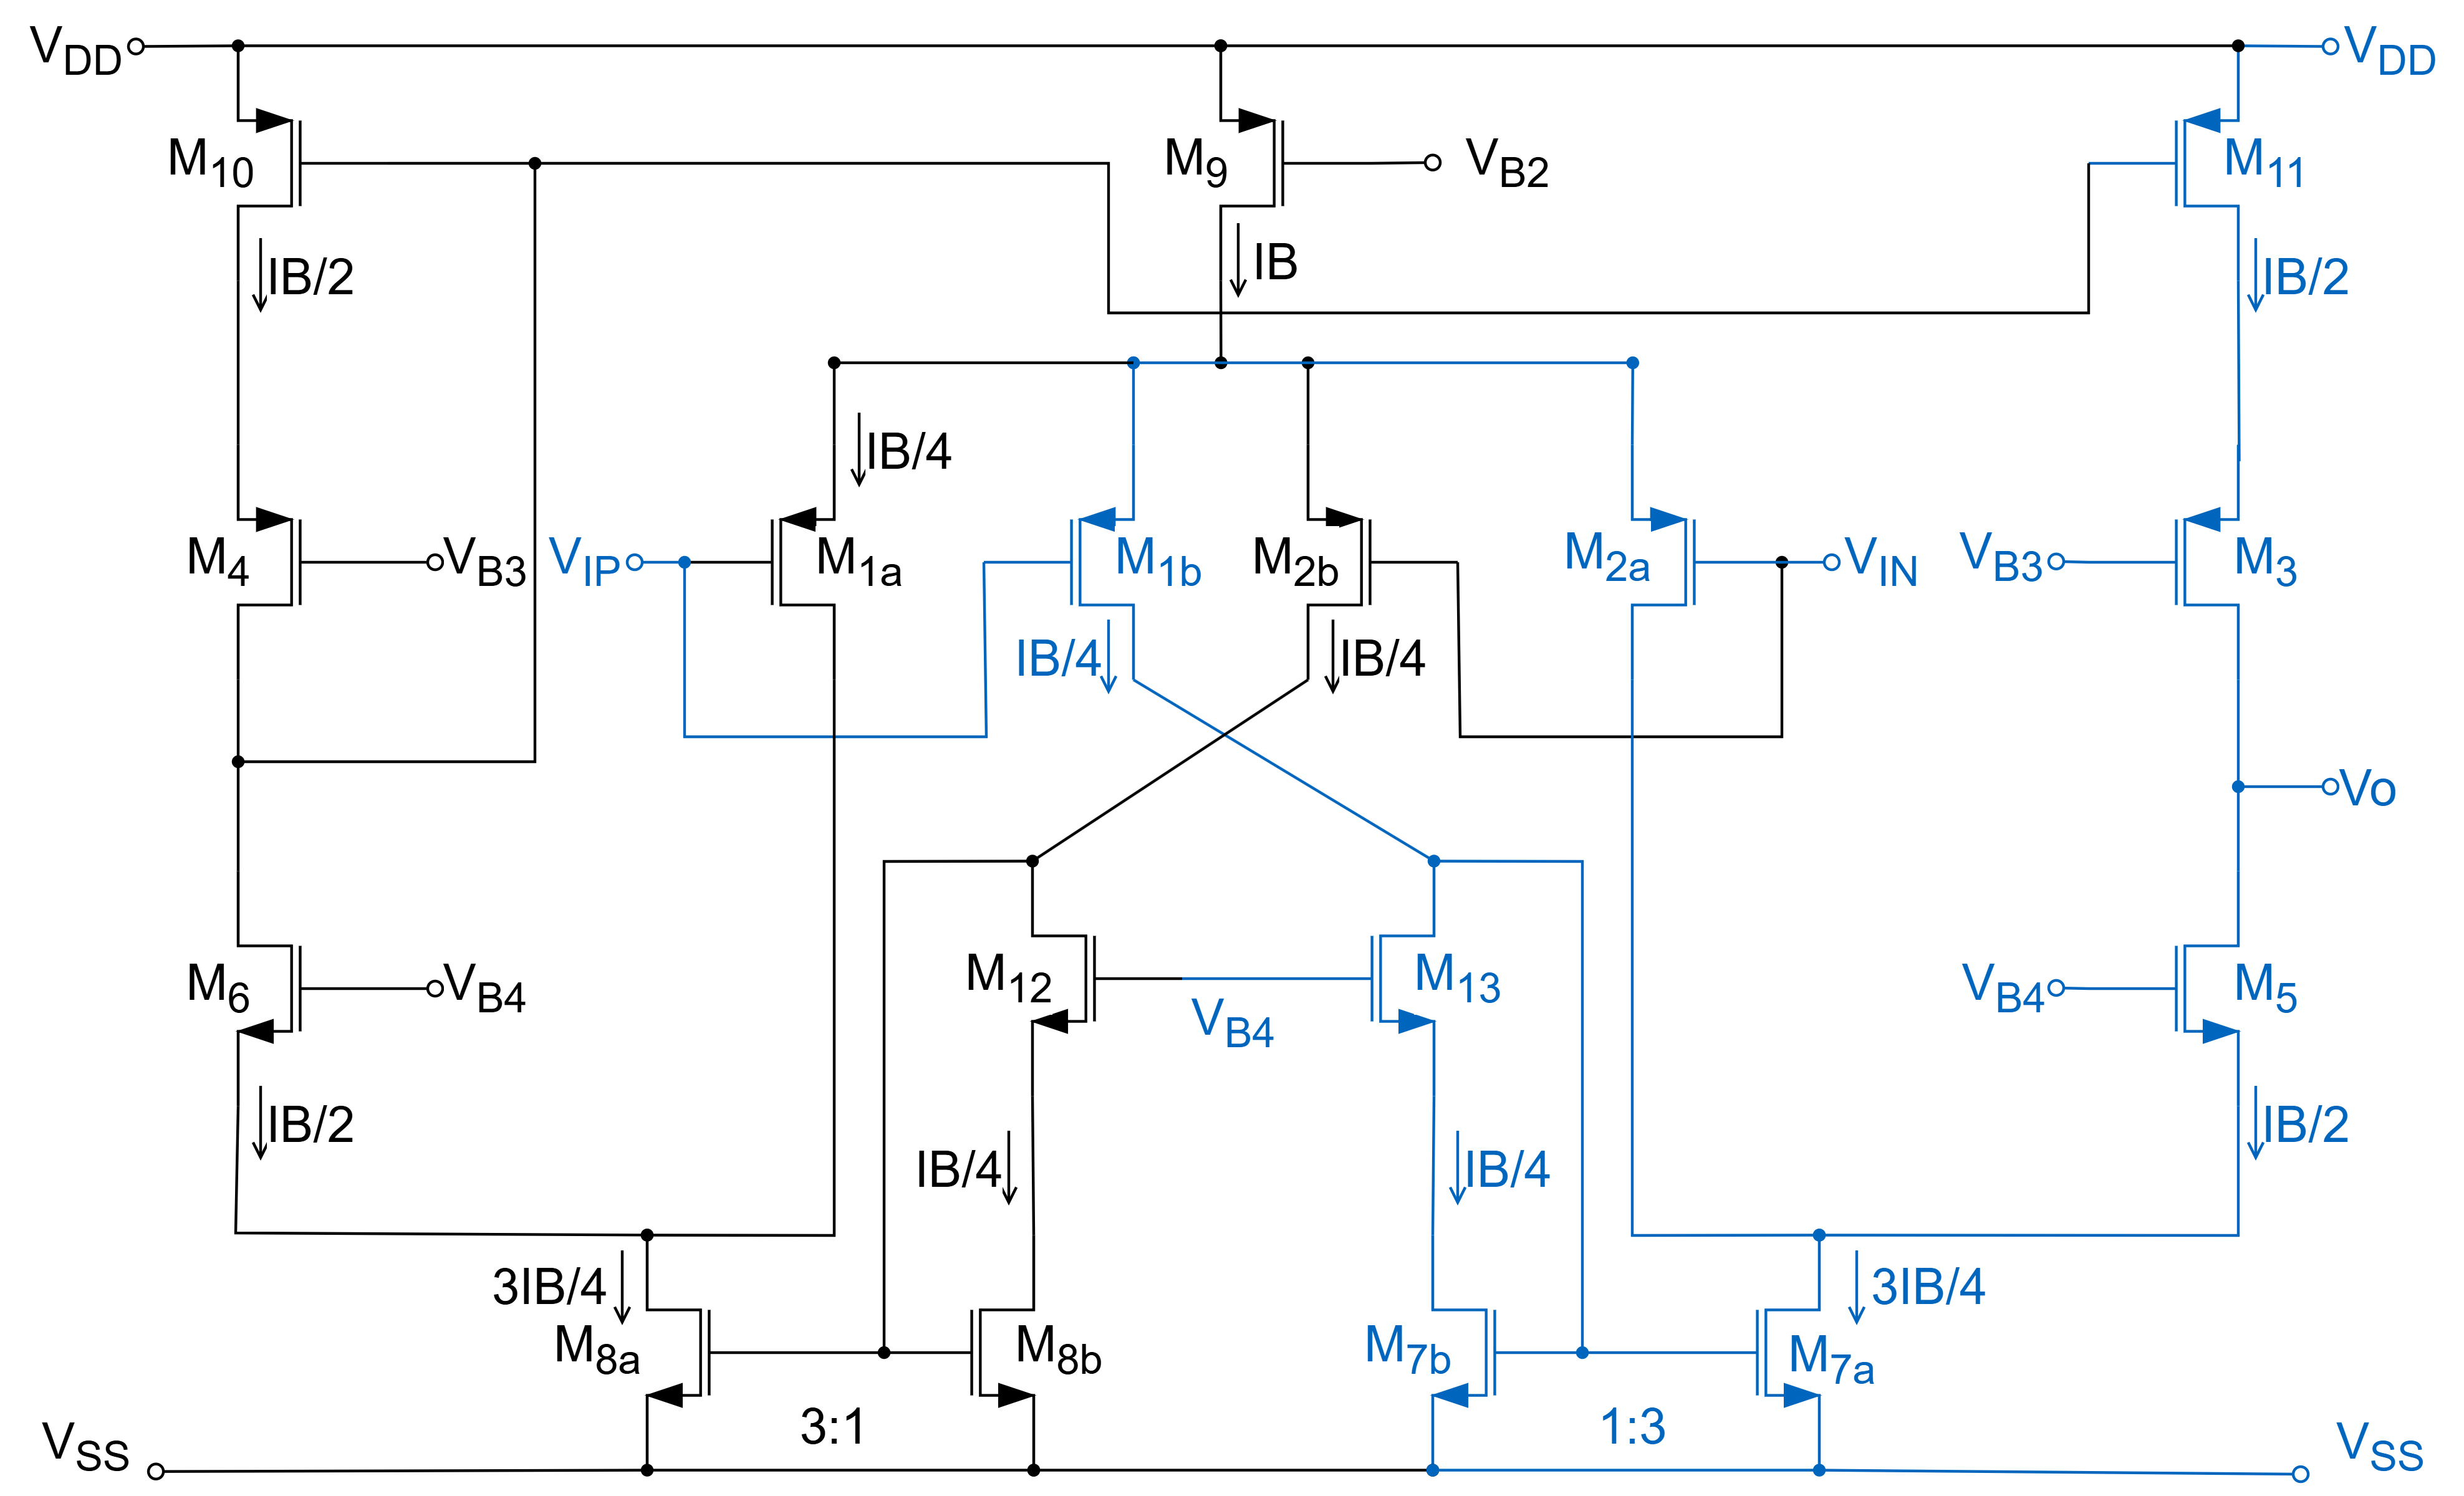
\includegraphics[width=1\textwidth]{Images/full_sch.png}
    \caption{Full Schematic without biasing circuit}
    \label{fig:full_schematic}
\end{figure}

For sake of simplicity, the theoretical analysis was done only in half of the circuit, as showed in Figure \ref{fig:simplified_schematic}. The analysis was done in the half that contains the output signal, and as the other half is symmetrical to the one analyzed, the results obtained in this analysis can be applied to the both halves of the circuit. 

The parameters chosen to study were based on the constraints and goals mentioned in Table \ref{tab:goals}. The following subsections will explain how the values for the different parameters were obtained.

\textcolor{red}{explicar os main blocos do circuito ir ver o artigo}

\begin{figure}[H]
    \centering
    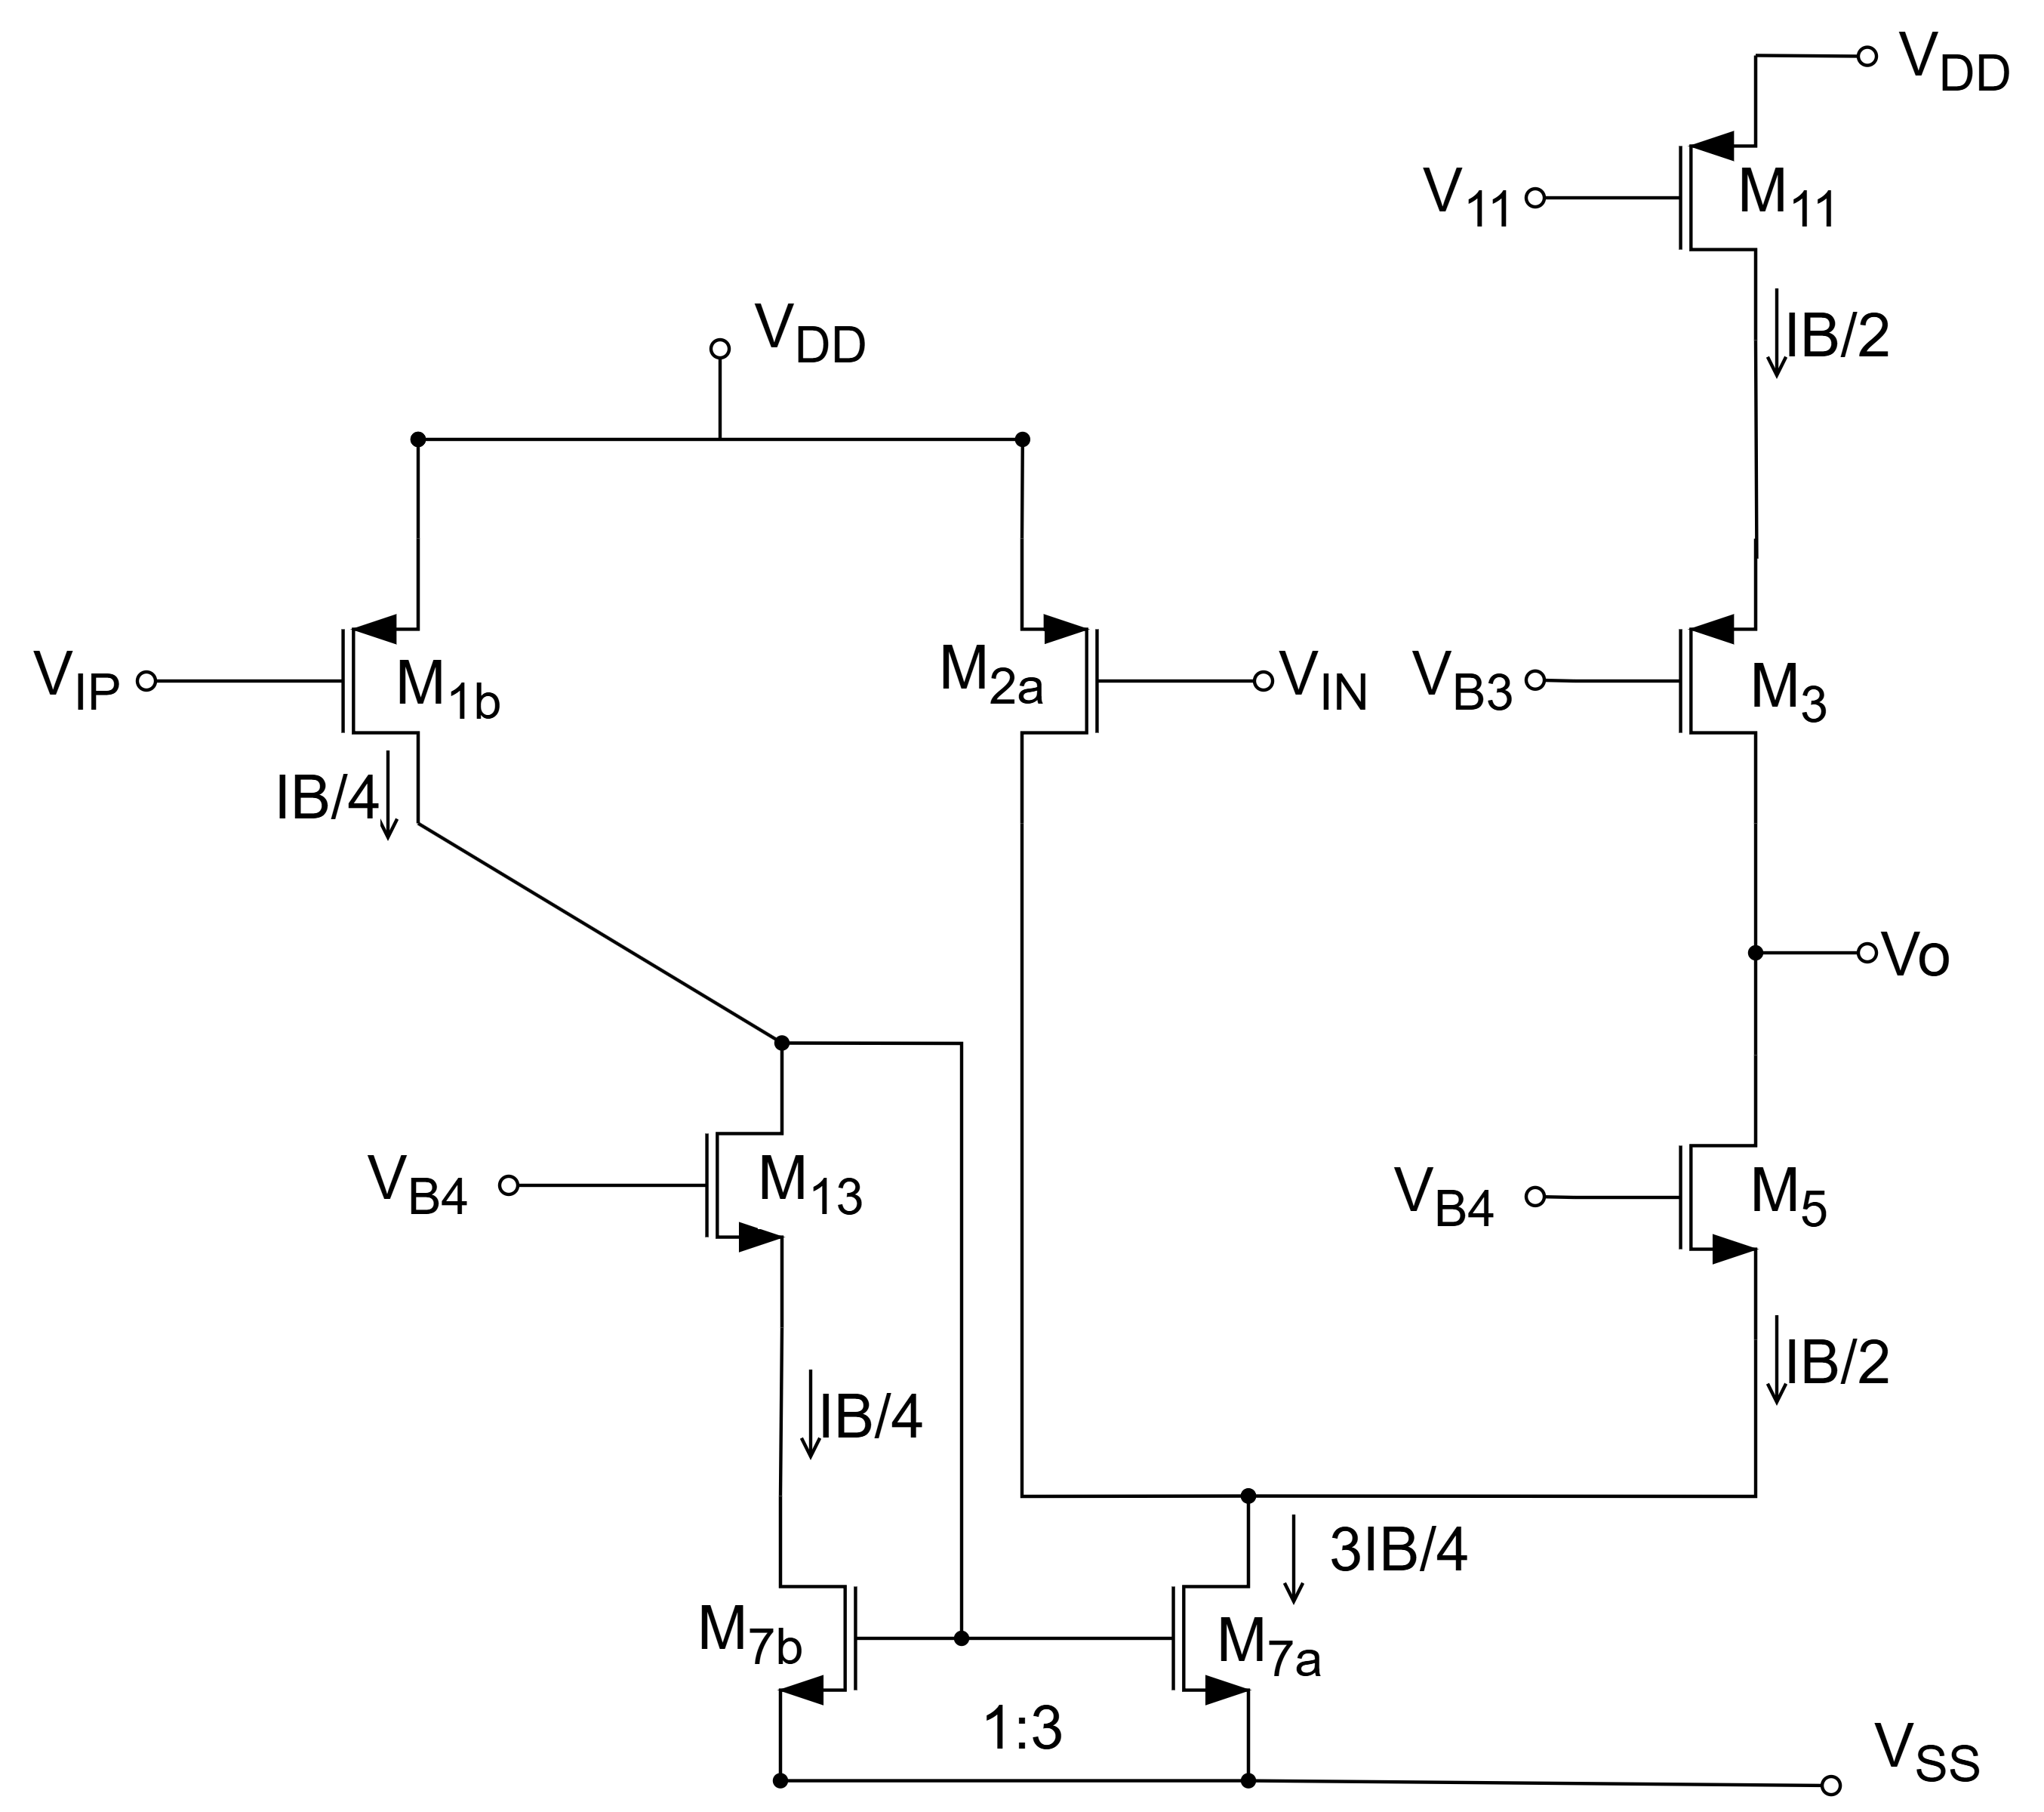
\includegraphics[width=0.6\textwidth]{Images/simplified_sch.png}
    \caption{Simplified Schematic}
    \label{fig:simplified_schematic}
\end{figure}

\subsection {DC Gain}

The DC gain $A_v$ is obtained as the short-circuit transconductance $G_M$ multiplied by the output resistance $r_{out}$.

$$A_v = G_M \cdot r_{out}\ [V/V]$$

The short-circuit transconductance $G_m$, that is represented in Figure \ref{fig:cc_transconductance} is calculated analysing the small signals model dipicted in Figure \ref{fig:small_signals}.

\begin{figure}[H]
    \centering
    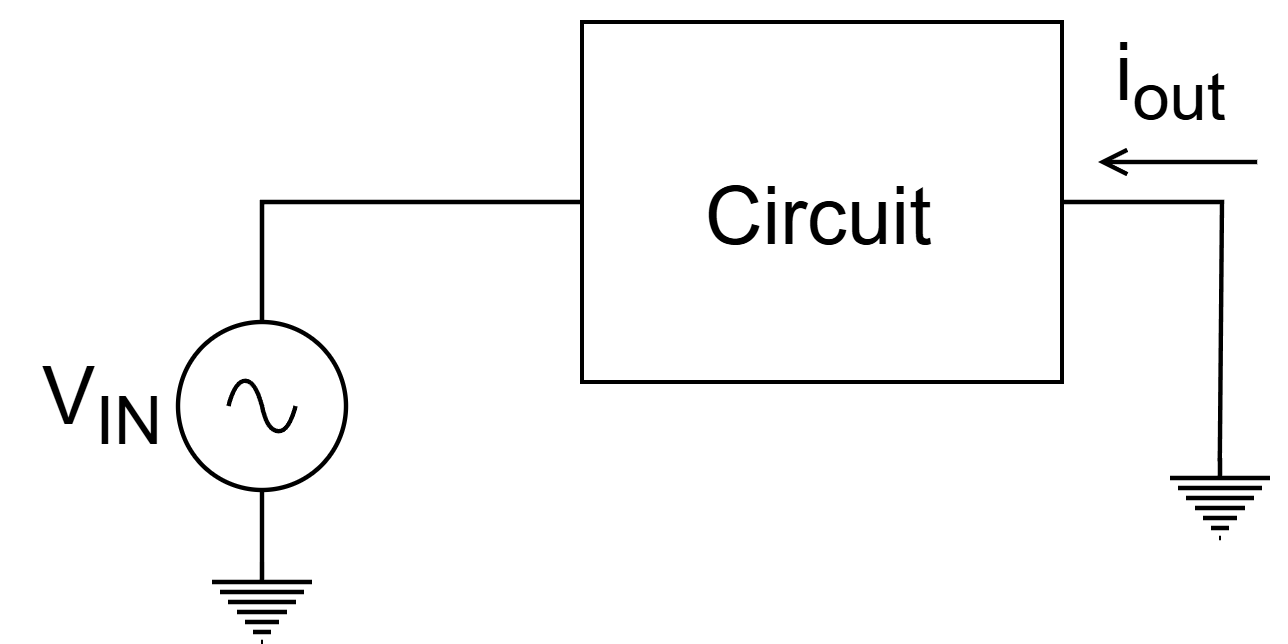
\includegraphics[width=0.4\textwidth]{Images/cc_transconductance.png}
    \caption{Short-circuit transconductance calculation diagram}
    \label{fig:cc_transconductance}
\end{figure}

\begin{figure}[H]
    \centering
    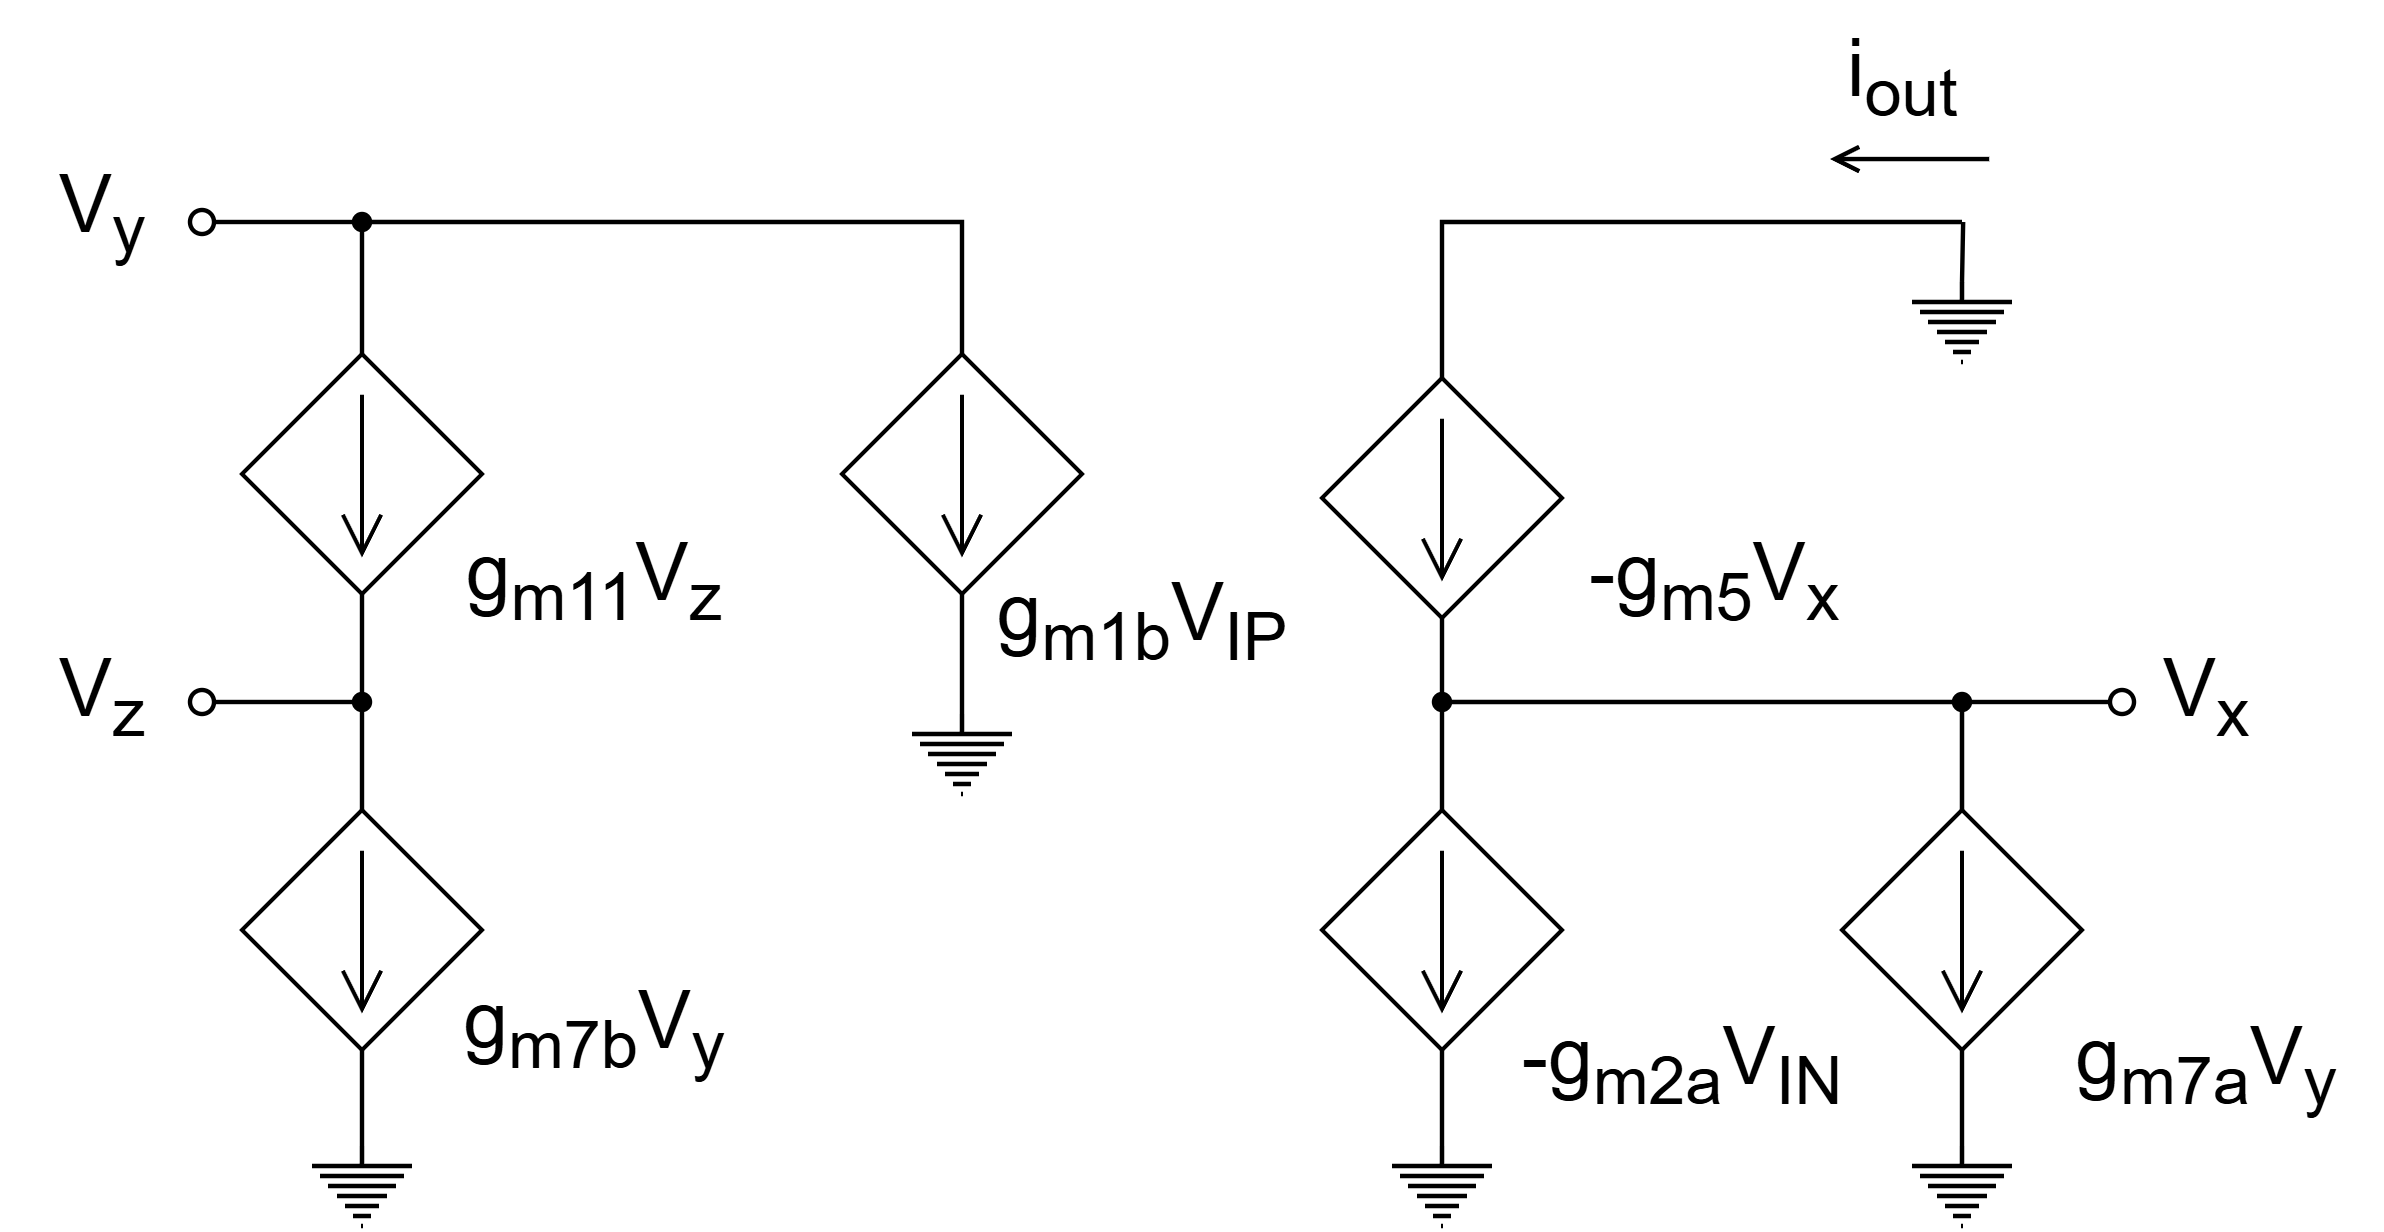
\includegraphics[width=0.7\textwidth]{Images/small_signals.png}
    \caption{Small signals model}
    \label{fig:small_signals}
\end{figure}

The transconductance $G_M$ is given by:
\begin{equation}
G_M = \left. \frac{i_{\text{out}}}{v_{\text{ip}}} \right|_{v_{\text{out}}=0} \ [\Omega ^{-1}] \\
\label{eq:Gm_general}
\end{equation}

Applying KCL in the nodes and manipulating the equations, the following expression for $G_M$ is obtained:

\begin{equation}
    G_M = g_{m2a} + g_{m1b} \cdot \frac{g_{m7a}}{g_{m7b}} \ [\Omega ^{-1}] \\
    \label{eq:GM_symbols}
\end{equation}

Since the relation between $g_{m7a}$ and $g_{m7b}$ is given by $g_{m7a} = 3 \cdot g_{m7b}$, the expression for $G_m$ can be simplified to:  

\begin{equation}
    G_M = BE \cdot (g_{m2a} + 3 \cdot g_{m1b}) \ [\Omega ^{-1}] \\
    \label{eq:GM_BE}
\end{equation}

The constant BE was added to simulate the body effect present on those transistors.

Studying the output resistance $r_{out}$, in can be seen as:

\begin{equation}
    r_{out} = \frac{1}{g_{out}} \ [\Omega] \\
    \label{eq:rout}
\end{equation}

The output conductance $g_{out}$ is given by:

\begin{equation}
    g_{out} = g_{op} + g_{on} \ [\Omega ^{-1}] \\
    \label{eq:gout}
\end{equation}

Where $g_{op}$ is the conductance seen from the output node to the upper part of the circuit $V_{dd}$ and $g_{on}$ is the conductance seen from the output node to the lowest part of the circuit $V_{ss}$.

\begin{equation}
    \begin{cases}
        g_{op} = g_{ds11} \cdot \frac{g_{ds3}}{g_{m3}} \\
        g_{on} = \left( g_{ds2a} + g_{ds7a} \right) \cdot \frac{g_{ds5}}{g_{m5}}
    \end{cases}
    \label{eq:output_conductance}
\end{equation}

The DC gain $A_v$ is given by:

\begin{equation}
    |A_v| = \frac{G_m}{g_{on} + g_{op}} = \frac{BE \cdot (g_{m2a} + 3 \cdot g_{m1b})}{g_{ds11} \cdot \frac{g_{ds3}}{g_{m3}\cdot BE} + (g_{ds2a} + g_{ds7a}) \cdot \frac{g_{ds5}}{g_{m5} \cdot BE}} \ [V/V]
    \label{eq:Av}
\end{equation}

As mentioned before, the constant BE was added to simulate the body effect present on those transistors.

\subsection{Gain Bandwidth Product (GBW)}
The gain bandwidth product is denoted by the product of the DC gain $A_v$ and the dominant pole frequency $f_{po}$, that is the frequency where the gain of the amplifier is 0 dB. 

The dominant pole frequency $f_{po}$ is given by:

\begin{equation}
    f_{po} = \frac{1}{2\pi \cdot r_{out} \cdot C_{out}} \ [Hz]
    \label{eq:fpo}
\end{equation}

The gain bandwidth product is given by:

\begin{equation}
    GBW = \frac{A_v}{f_{po}} = \frac{G_M \cdot r_{out}}{2\pi \cdot C_{out} \cdot r_{out}}=\frac{G_M}{2\pi \cdot C_{out}} \ [Hz]
    \label{eq:GBW}
\end{equation}

$C_{out}$ is depicted in Figure \ref{fig:cout_sch} and is given by :

\begin{equation}
    C_{out} = C_L + C_{bd3} + C_{gd3} + C_{bd5} + C_{gd5} \ [F]
    \label{eq:cout}
\end{equation}

\begin{figure}[H]
    \centering
    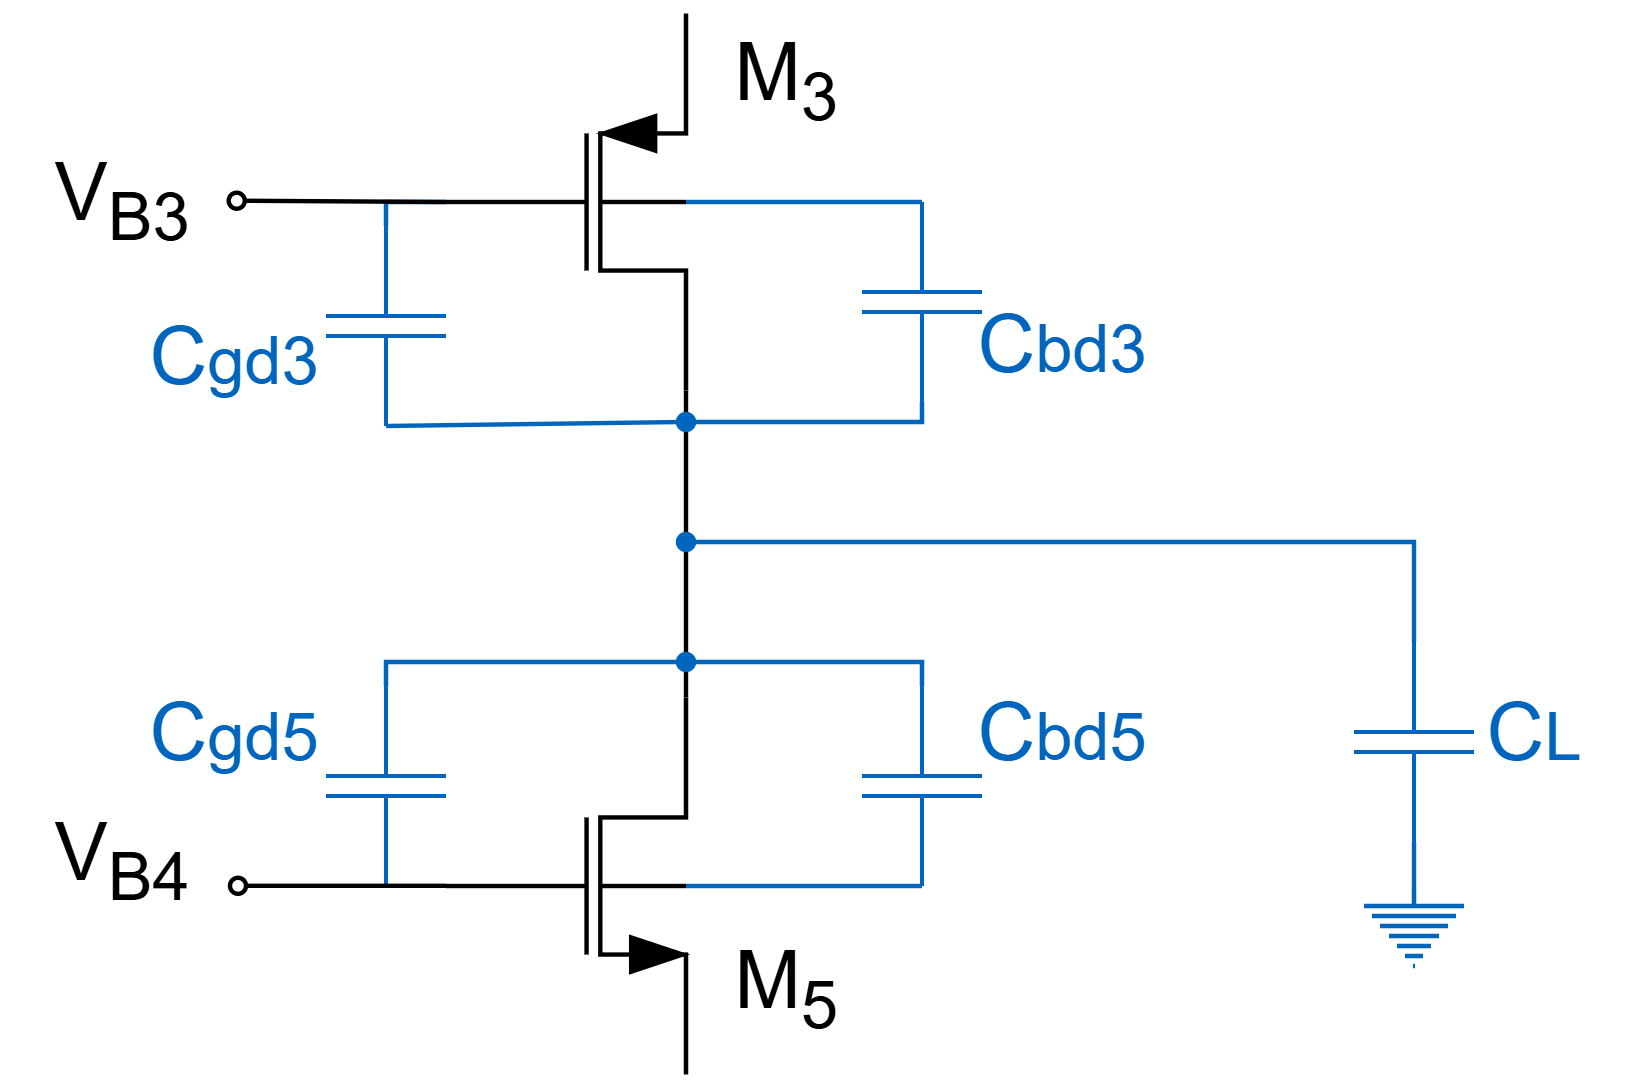
\includegraphics[width=0.5\textwidth]{Images/Cout_sch.png}
    \caption{Output capacitance calculation schematic}
    \label{fig:cout_sch}
\end{figure}

\subsection{Second and Third Pole Frequencies}
In order to guarantee stability in a unity-gain closed-loop configuration the four remaining poles were studied. At this stage the second and third pole frequencies are not defined because they vary with the transistors specifications. Thus, in this subsection were calculated all the pole frequencies to further analyze the stability of the amplifier. 

The pole frequencies are given by:

\begin{align}
    f_{px} &= \frac{1}{2\pi \cdot C_x \cdot r_x} \ [Hz] &
    f_{py} &= \frac{1}{2\pi \cdot C_y \cdot r_y} \ [Hz] \\
    f_{pz} &= \frac{1}{2\pi \cdot C_z \cdot r_z} \ [Hz] &
    f_{p7} &= \frac{1}{2\pi \cdot C_w \cdot r_w} \ [Hz]
    \label{eq:poles}
\end{align}

\begin{figure}[H]
    \centering
    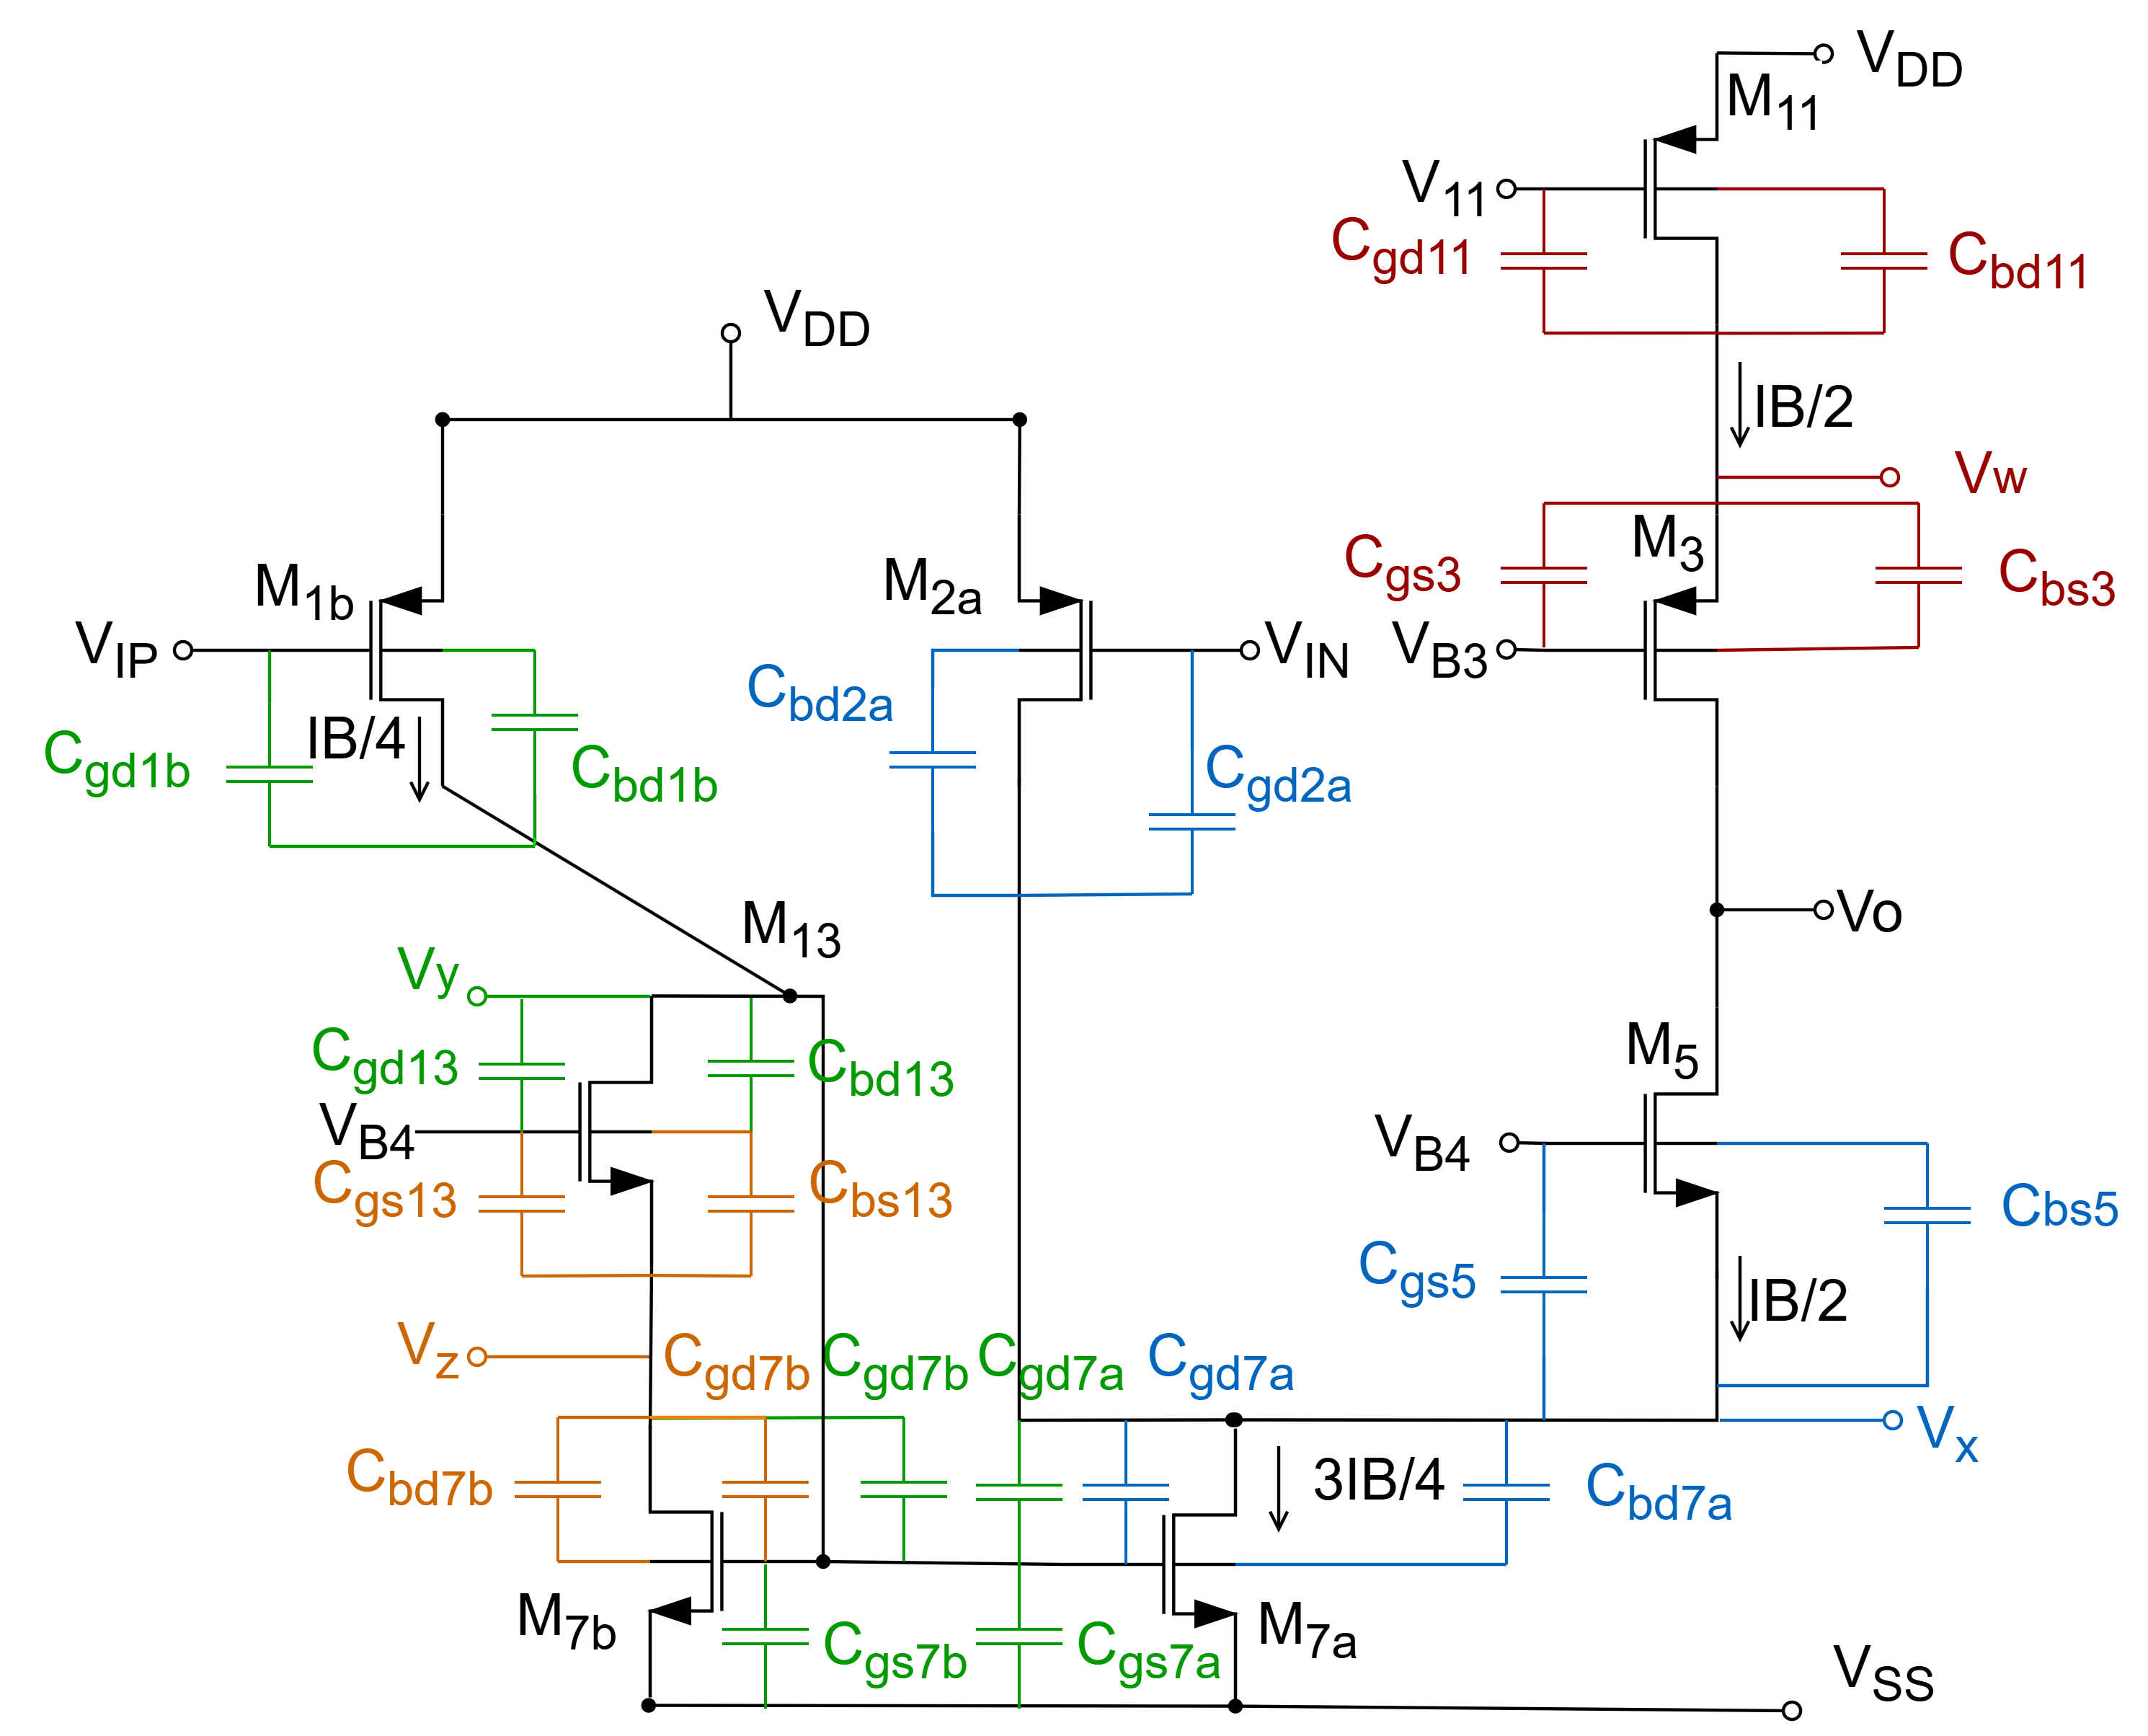
\includegraphics[width=0.8\textwidth]{Images/pole_freqs.png}
    \caption{Capacitances calculation schematic}
    \label{fig:poles_sch}
\end{figure}

Thus, we will need to calculate the equivalent capacitances at node $x$, $y$, $w$ and $z$, depicted in Figure \ref{fig:poles_sch}, are given by:

\begin{align}
    C_x &= C_{gd7a} + C_{bd7a}+ C_{gd2a} + C_{bd2a} + C_{gs5} + C_{bs5} \ [F] \\
    C_y &= C_{gd1b} + C_{bd1b} + C_{gd13} + C_{bd13} + C{gd7b} + C_{gs7b} + C{gd7a} + C_{gs7a}\ [F] \\
    C_w &= C_{gd11} + C_{bd11} + C_{bs3}+ C_{gs3} \ [F] \\
    C_z &= C_{gs13} + C_{bs13} + C_{bd7b}+ C_{gd7b} \ [F] 
    \label{eq:capacitances}
\end{align}
\\
The equivalent resistances at nodes in study are given by:

\begin{align}
    r_x &= \frac{1}{g_{m5}} \ // \ \frac{1}{g_{ds7a}} \ // \ \frac{1}{g_{ds2a}}\approx \frac{1}{g_{m5} \cdot BE} \ [\Omega]\\
    r_y &= \frac{1}{g_{ds1b}} \ // \ \frac{1}{g_{m7b}} \approx \frac{1}{g_{m7b}} \ [\Omega]\\
    r_w &= \frac{1}{g_{ds11}} \ // \ \frac{1}{g_{m3}} \approx \frac{1}{g_{m3} \cdot BE} \ [\Omega]\\
    r_z &= \frac{1}{g_{m13}} \ // \ \frac{1}{g_{ds7b}} \approx \frac{1}{g_{m13} \cdot BE} \ [\Omega]
    \label{eq:resistances}
\end{align}

\subsection{Output Swing}
The output-swing defines the maximum approximation of the amplifier's output voltage to the supply voltages ($V_{dd}$ and $V_{ss}$), to prevent saturation. The output-swing takes into account the voltages needed to keep the output transistors in the moderate inversion zone and also the operating margin, which in this case is $V_{margin}=80mV$ for each side.

The output-swing of the amplifier can be obtained by the following expression:
\begin{equation}
    OS = V_{DD} - V_{DSsat11} - V_{DSsat3} - V_{DSsat5} - V_{DSsat7a} - 0.16 \ [V]
    \label{eq:OS}
\end{equation}

\subsection{Excess-Noise Factor}
The Excess-Noise factor is the additional noise created by an amplifier with gain $A_v$. An amplifier with excess noise of 1 means that the intrinsic noise is multiplied by 1 therefore, the noise is not made any worse, but any value over 1 means the noise is increased due to the gain.

The amplifier's excess noise factor was studied for only half of the circuit. Bearing in mind that in cascode configurations the common-gate transistors do not generate noise because they cannot impose current on the circuit, the value for Excess-Noise factor $\Gamma$ is given by the following equation:

\begin{equation}
    \Gamma = 1 + \frac{3}{4}\cdot \frac{gm_{7a}}{gm_{2a}} + \frac{1}{4}\cdot \frac{gm_{11}}{gm_{2a}} \ [\Omega ^{-1} / \Omega ^{-1}]
    \label{eq:ENF}
\end{equation}


\subsection{Power Dissipation}

Its intended that the power dissipation $P_D$ is minimized in order to have the best performing low power amp.

Where: 
\begin{equation}
    P_D = V_{DD} \times \left(2 \times I_B + \dfrac{I_B\cdot 4}{10}\right) \ [W]
    \label{eq:PD}
\end{equation}

\subsection{Figure of Merit (FoM)}
 We will also need to achieve the best possible figure-of-merit FoM defined by: 
\begin{equation}
    FoM = \frac{GBW \times C_L}{P_D} \ [MHz \cdot pF/mW]
    \label{eq:FoM}
\end{equation}
